\documentclass[../../main.tex]{subfiles}
\begin{document}
\graphicspath{{./figures}}
\chapter{Análisis de la cadena de RF}

La definición de la especificación de la cadena de RF es una parte fundamental en el diseño del receptor. 
Para todos los cálculos realizados en este capítulo se tomó como referencia la misión BEESAT-9 \cite{BEESAT-9} de la Universidad de Berlín. 
La razón de esta elección radica en que se trata de un satélite LEO a $h_\textrm{sat} = 530\un{km}$ de altura el cual opera en la banda de interés de UHF amateur, más específicamente a una frecuencia central $f_0 = 435.95\un{MHz}$.

\section{Planteo del front-end de RF}
Un esquema simplificado del \textit{front-end} de RF se presentó ya en la figura \ref{fig::front-end-rf-16}, una ilustración más detallada  se muestra en la figura \ref{fig::cadena-de-recepcion}. Allí se observa que se compone de los siguientes elementos:
\begin{itemize}
    \item Un tramo de cable de aproximadamente 50~cm desde los elementos radiantes hasta el híbrido.
    \item Un híbrido en cuadratura el cual combina dos elementos radiantes lineales para lograr una polarización circular.
    \item Un tramo de 5~cm de cable aproximadamente, el cual conecta el híbrido con el resto de la cadena de RF.
    \item Un filtro grueso preselector de 25~MHz de ancho de banda para proteger al LNA evitando que sature y, además, realizar una selección gruesa de la banda de interés.
    \item Un LNA de 27~dB de ganancia. Su figura de ruido determina la del sistema por ley de Friis, es por esto que es relevante minimizarla.
    \item Un tramo de cable de aproximadamente 2 metros para conectar con el resto del sistema.
    \item Una etapa de gran ganancia $G$, la cual acondiciona la potencia de la señal de manera de cumplir con los requerimientos del demodulador. Esta es la ganancia a determinar en este análisis.
    \item Un último tramo de cable de alrededor de 30~cm para conectar el final de la cadena de recepción a la entrada del sistema de adquisición.
\end{itemize}

Como se mencionó anteriormente, la figura de ruido del \textit{front-end} de RF estará determinada principalmente por el LNA. Dado que su caracterización no es una tarea propia del presente proyecto, se considerará para este análisis $\textrm{NF}_\textrm{FE} = 3\un{dB}$ que representa un valor estimativo.

\figura[0.7]{cadena-de-recepcion}{Diagrama de la cadena de recepción.}
\unsure{Debería agregar ganancias a aplificadores y longitudes a cables?}
\change{Sacar el ADC. Señalizar que la NF es de aprox 3 dB}
\section{Análisis de potencia} 
Se comenzó realizando un análisis de potencia en la antena receptora con el objetivo de determinar la SNR de partida para luego, en base a esta, realizar los cálculos subsiguientes para la determinación de la ganancia $G$. La potencia en la antena receptora viene dada por la ecuación \ref{eq::potencias}:

\begin{equation}
    P_\textrm{ant} = P_\textrm{sat} - L_\textrm{FS} - L_\textrm{pol} + G_\textrm{el} (\theta),
    \label{eq::potencias}
\end{equation}
donde $P_\textrm{ant}$ es la potencia recibida en la antena del receptor, 
$P_\textrm{sat} = 27~\un{dBm}$ es la potencia transmitida por la misión de referencia, $L_\textrm{FS} = 20 \log \left(\frac{4 \pi d}{\lambda}\right)$ representa las pérdidas de espacio libre, $L_\textrm{pol} = 3~dB$
 son las pérdidas por polarización ya que la misión de referencia transmite en polarización lineal (y la recepción se realiza con polarización circular, ver figura \ref{fig::cadena-de-recepcion}), y $G_\textrm{el} (\theta)$ es la ganancia por elemento para un dado ángulo.

La distancia $d$ empleada para calcular $L_\textrm{FS}$ representa la distancia del satélite al arreglo de antenas y puede aproximarse mediante el teorema del coseno para un ángulo de elevación $\theta$ respecto al horizonte a partir de la ecuación \ref{eq::distSatelite}:
\begin{equation}
    (r_e + h_\textrm{sat})^2 = d^2 + r_e^2 - 2 d r_e \cos{(90\degree + \theta)},
    \label{eq::distSatelite}
\end{equation}
donde $r_e = 6371\un{km}$ es el radio promedio de la Tierra.

A continuación se calculó la SNR a la entrada del receptor como la resta en dB de la potencia de señal en la antena receptora dada por la ecuación \ref{eq::potencias} y la potencia de ruido en el ancho de banda de entrada dada por la ecuación \ref{eq::potenciaRuido}:
\begin{equation}
    N = N_0 B = k T_\textrm{ant} \cdot 25\un{MHz},
    \label{eq::potenciaRuido}
\end{equation} 
donde $k$ es la constante de Boltzmann, $T_\textrm{ant}$ la temperatura de la antena receptora y $B = 25\un{MHz}$ es el ancho de banda del primer filtro grueso de la cadena de recepción mostrada en la figura \ref{fig::cadena-de-recepcion}.

Se consideraron dos configuraciones extremas para cubrir los posibles rangos de valores de $L_\textrm{FS}$ y $G_\textrm{el}(\theta)$. 
La primera de estas corresponde al considerado el peor caso; el cual se tiene al al arreglo a $45\degree$ y el satélite se encuentra a $10\degree$ sobre la línea del horizonte como se observa en la figura \ref{fig::peor-caso}

Por otro lado, la segunda configuración analizada representa el mejor caso, esto es, aquel en el cual el arreglo de antenas se encuentra horizontal sobre la tierra y el satélite se posiciona en el zénit como se muestra en la figura \ref{fig::mejor-caso}.

\begin{figure}[H]
    \centering
    \subcaptionbox{Peor caso considerado.\label{fig::peor-caso}}
    {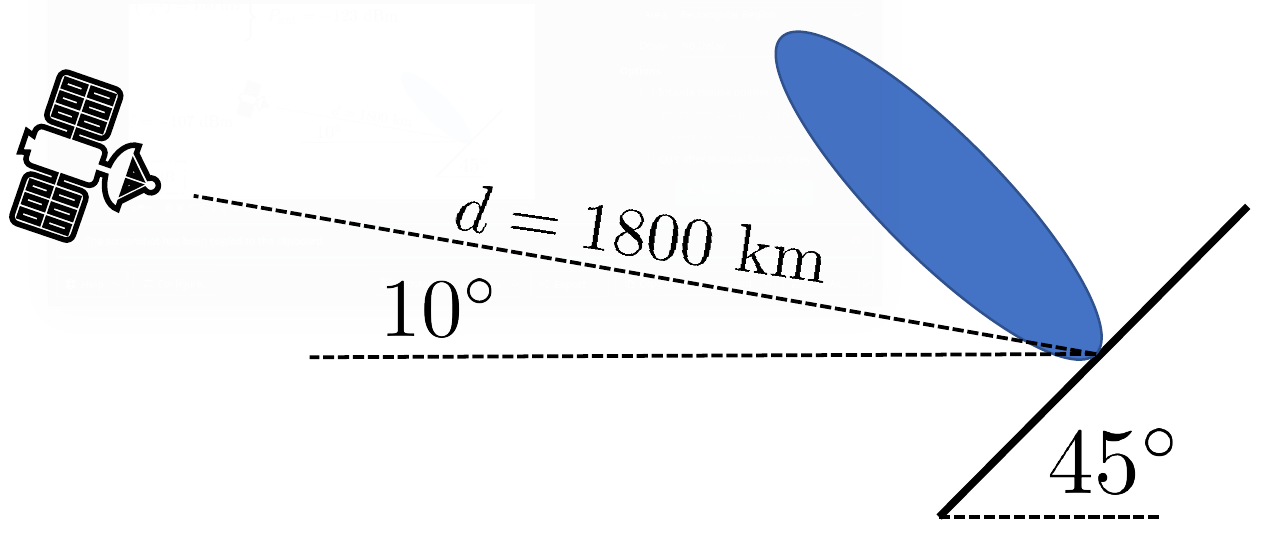
\includegraphics[width=0.7\linewidth]{peor-caso.png}}\\[1PC]
    \subcaptionbox{Mejor caso considerado.\label{fig::mejor-caso}}
    {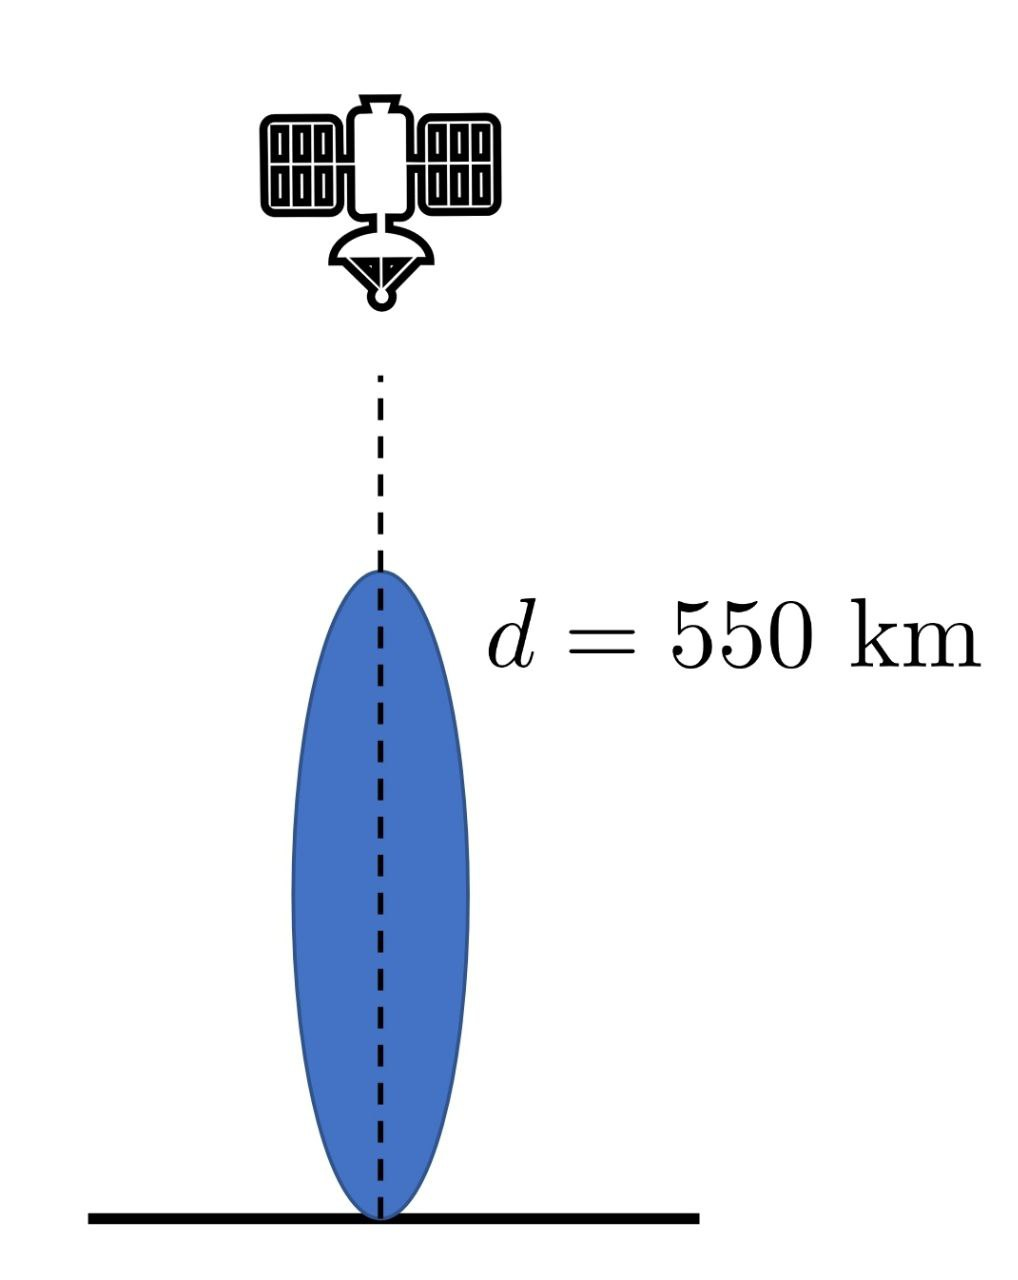
\includegraphics[width=0.45\linewidth]{mejor-caso.jpg}}
    \caption{Escenarios considerados en el análisis de potencia.}
    \label{fig::casos-potencia}
\end{figure}

\subsection{Evaluación del peor caso}
Para la configuración mostrada en la figura \ref{fig::peor-caso}, la distancia de la misión de referencia al satélite según la ecuación \ref{eq::distSatelite} es de aproximadamente $1800\un{km}$. Esta distancia se calcula a partir de la ecuación \ref{eq::distSatelite} y representa unas pérdidas de espacio libre de $L_\textrm{FS} = 150\un{dB}$. 
Por otro lado, la ganancia de cada elemento en estas condiciones fue determinado mediante simulaciones \unsure{Lo pongo en el apéndice? Ver docs de Nico}, donde se obtuvo $G_\textrm{el}(10\degree) = 3\un{dBi}$. Al sustituir los valores recién obtenidos en la ecuación \ref{eq::potencias} se obtiene que la potencia de señal que alcanza a cada elemento es $P_\textrm{ant} = -123\un{dBm}$.

Para calcular la potencia de ruido empleando la ecuación \ref{eq::potenciaRuido} se debe determinar la temperatura de ruido de la antena\footnote{Esto es de cada elemento, no del arreglo entero.}.
\todo{Poner como se determinó la temperatura de la antena.}
\todo{Poner la SNR obtenida restando los valores y labelar la eq}

\subsection{Evaluación del mejor caso}
El segundo caso extremo a analizar es el mostrado en la figura \ref{fig::mejor-caso}. La distancia de la misión de referencia al arreglo es simplemente su altura $h_{sat}$, esto es 550~km, lo cual implica unas pérdidas de espacio libre de $L_\textrm{FS} = 140\un{dB}$. La ganancia de cada elemento en este escenario es $G_\textrm{el}(90\degree) = 8\un{dBi}$. Así, la potencia de señal a la entrada de cada elemento es $P_\textrm{ant} = -108\un{dBm}$.

Para esta configuración, la temperatura de cada antena es
\todo{Poner como se determinó la temperatura de la antena.}
\todo{Poner la SNR obtenida restando los valores y labelar la eq}

\section{Ruido introducido por el ADC}
El conversor analógico-digital es un dispositivo complejo con numerosas fuentes de ruido \cite{ruidos-adc}. En este análisis se consideran las tres fuentes principales en términos del nivel de ruido aportado en la frecuencia de trabajo de la misión de referencia \cite{AD9249}. Estas son:
\begin{itemize}
    \item Ruido térmico.
    \item Ruido de cuantización.
    \item Ruido por \textit{jitter}.
\end{itemize}

\subsection{Ruido térmico}
En la figura \ref{fig::ruido-termico} se muestra la SNR en dBFS en función de la frecuencia. Se observa que, para el caso bajo análisis de $f_0 = 435.95\un{MHz}$, la SNR es de aproximadamente 65~dBFS. Esto implica que el ruido térmico o ruido Johnson en dBFS es de -65~dBFS. Esto es:
\begin{equation}
    N_T = -65\un{dBFS}
    \label{eq::ruido-termico}
\end{equation}

\figura[0.65]{ruido-termico}{SNR del AD9249 en función de la frecuencia de entrada \cite{AD9249}.}

\subsection{Ruido de cuantización}
Al muestrear una señal se discretiza una magnitud física, en este caso esta magnitud es la tensión. De esta manera, dado que con N bits se pueden representar hasta $2^N$ valores, se comete inevitablemente un error al realizar el muestreo de una variable continua; esto se ilustra en las figuras \ref{fig::cuantizacion} y \ref{fig::sampleo}. Dicho error recibe el nombre de error de cuantización.

Este error puede modelarse como una variable aleatoria con distribución uniforme en el intervalo $[-\textrm{FSR}/{2^{N_\textrm{b} + 1}}, \textrm{FSR}/{2^{N_\textrm{b} + 1}}]$ \cite{formula-cuantizacion}, donde $N_\textrm{b}$ es el número de bits efectivos del usados en el muestreo. Luego, para una señal de entrada sinusoidal \textit{full scale} se obtiene que la potencia de ruido de cuantización (que deriva del error de cuantización) puede calcularse de acuerdo a la siguiente fórmula \cite{formula-cuantizacion}:
\begin{equation}
    N_q = - (1.763 + 6.02 N_\textrm{b})\un{dBFS},
    \label{eq::ruido-cuantizacion-formula}
\end{equation}
\unsure{Lo de bits efectivos está relacionado con el oversampling, ver si lo dejo o no.}

El AD9249 posee una resolución de 14 bits como se indicó en la tabla \ref{tab::ADC}. Luego, de la ecuación \ref{eq::ruido-cuantizacion-formula}, el ruido de cuantización es:
\begin{equation}
    N_q = -86\un{dBFS}.
    \label{eq::ruido-cuantizacion}
\end{equation}

\figura[0.55]{cuantizacion}{Código de cuantización con 4 bits \cite{ruidos-adc}.}

\figura[0.55]{sampleo}{Señal analógica y señal muestreada junto con el error del bit menos significativo \cite{ruidos-adc}.}

\subsection{Ruido por \textit{jitter}}
Existen dos fuentes de incertidumbre en el momento de la conversión, el \textit{jitter} del reloj externo de muestreo y la incertidumbre en el tiempo de apertura del ADC, ambos valores se especifican en la table \ref{tab::ADC}.

Dado que se trata de efectos independientes, se calcula el \textit{jitter} $t_j$ resultante como la suma en cuadratura de ambos efectos:
\[t_j = \sqrt{{(1\un{ps})}^2 + {(135\un{fs})}^2} \approx 1\un{ps}\]

La potencia de ruido de \textit{jitter} para una entrada sinusoidal puede calcularse como \cite{formula-jitter}:
\begin{equation}
    N_j = 20 \log{\left(2 \pi  f_{\textrm{in}} t_j\right)}\un{dBc} = -51\un{dBc},
    \label{eq::jitter-formula}
\end{equation}
para $f_{\textrm{in}} = 435.95\un{MHz}$, la frecuencia de operación de la misión de referencia. Resulta relevante notar que, a diferencia del ruido térmico y el de cuantización analizados anteriormente, el ruido de \textit{jitter} se expresa en dBc, es decir, la potencia de ruido de \textit{jitter} siempre estará 51~dB por debajo de la potencia de portadora.

\subsection{SNR a la salida del ADC en función de la ganancia $G$}
El parámetro libre en este análisis es la ganancia $G$ de la segunda etapa de amplificación, la cual puede verse en la figura \ref{fig::cadena-de-recepcion}. Por esto resulta de relevancia analizar las implicancias que tiene la variación de este parámetro en el sistema.
Empleando \textit{full scale} como $1~V_\textrm{pp}$, se tiene que 
$$0\un{dBFS} \approx 4\un{dBm},$$ 
\unsure{Hace falta que explique de donde sale?} 
lo cual según las ecuaciones \ref{eq::ruido-termico} y \ref{eq::ruido-cuantizacion} implica que los ruidos térmico y de cuantizacion resultan:
\[N_T = -61\un{dBm},\] \[N_q = -82\un{dBm}.\]

En la figura \ref{fig::ruidovsG} se muestra la potencia en dBm de la señal de entrada y los términos de ruido del ADC y el ruido de RF para el peor caso de recepción (ver figura \ref{fig::peor-caso}) en función de la ganancia $G$. Se incluye además en dicho gráfico la suma en cuadratura de todos los términos\footnote{Se realiza la suma en cuadratura bajo la suposición de que estos efectos son independientes.} de ruido en representación del ruido total del sistema.

La SNR está representada en la figura \ref{fig::ruidovsG} por la diferencia entre $P_{in}$ y $N_{tot}$. Se observa a simple vista que aumentar el valor de $G$ mejora la SNR inicialmente hasta cierto punto donde la diferencia entre las curvas parece permanecer constante. Esto se ve con mayor claridad en la figura \ref{fig::SNRvsG} donde se grafica la SNR en función de la ganancia $G$ para el peor caso de recepción. Se ve que aumentar la ganancia $G$ por encima de los 55~dB no representa mejoras a la SNR.

\figura[0.7]{ruidovsG}{Potencia en dBm en función de la ganancia para la señal de entrada, los términos de ruido generados por el ADC y la suma en cuadratura de estos últimos. Se tomó como entrada una senoidal de 1~$V_\textrm{pp}$.}

\figura[0.7]{SNRvsG}{Relación señal a ruido en función de la ganancia $G$.}
\change{Sacar las líneas rojas}

\section{Determinación de la ganancia de la cadena de acondicionamiento}
El parámetro libre en este análisis es la ganancia $G$ de la segunda etapa de amplificación, la cual puede verse en la figura \ref{fig::cadena-de-recepcion}. Para determinar este parámetro se debe definir algún criterio de diseño, en el presente análisis este rol lo cumple la tasa de error de bit (BER) a la salida del demodulador. Se platea obtener una BER de $10^{-5}$.

El procedimiento a seguir para hallar el rango de posibles valores para G se ilustra en la figura \ref{fig::G-procedimiento} y puede describirse de la siguiente manera:
\begin{enumerate}
    \item Fijar un valor de BER a la salida del demodulador.
    \item Calcular la SNR requerida a la entrada del demodulador en base a la BER definida.
    \item Obtener la SNR requerida a la salida del ADC para la BER definida.
    \item Calcular la SNR a la salida del ADC en función del parámetro G.
    \item Sabiendo la SNR requerida y \change{Mejorar esta redacción}
\end{enumerate}

\figura[0.9]{G-procedimiento}{Partiendo de la BER como criterio de diseño, se propaga la SNR hacia atrás.}

\subsection{Requerimiento de SNR a la entrada del demodulador}
La relación señal a ruido (SNR) puede calcularse a través del parámetro $\frac{E_b}{N_0}$, esto es, el cociente entre la energía de bit y la densidad espectral de ruido a partir de la ecuación \ref{eq::EbN02SNR}:
\begin{equation}
    \textrm{SNR} = \frac{E_b}{N_0} \cdot \frac{R_b}{B},
    \label{eq::EbN02SNR}
\end{equation}
donde $R_b$ es la tasa de bits y $B$ es el ancho de banda ocupado.

Habiendo fijado la BER objetivo de $10^{-5}$ a la salida del demodulador, el siguiente paso es determinar la SNR requerida a la entrada del mismo. Esto depende del esquema de modulación utilizado que, en el caso de la misión de referencia, es GMSK. Para este esquema de modulación, la probabilidad de error de bit en presencia de RABG se relaciona con $\frac{E_b}{N_0}$ mediante la ecuación \ref{eq::BER2EbN0} \cite{haykin}:

\begin{equation}
    \textrm{BER} = \frac{1}{2} \textrm{erfc}\left(\sqrt{\frac{\alpha E_b}{2 N_0}}\right),
    \label{eq::BER2EbN0}
\end{equation}
donde $\alpha$ es un factor de degradación respecto a MSK, el cual depende del producto entre tiempo de bit ($T_b$) y ancho de banda ocuapado ($B$) del esquema GMSK. La degradación viene dada por la ecuación \ref{eq::degradacion},
\begin{equation}
    \textrm{Degradación} = 10 \log_{10}{\left(\frac{\alpha}{2}\right).}
    \label{eq::degradacion}
\end{equation}
En la figura \ref{fig::degradacion-bt} se muestra la degradación de la BER en función del producto $B T_b$ ($W T_b$ en inglés).

Para la misión de referencia, el factor de ancho de banda por tiempo de bit es $BT_b = 0.3$ \cite{BEESAT-9}. A partir de la figura \ref{fig::degradacion-bt} se observa que este factor corresponde con una degradación de aproximadamente $0.5\un{dB}$, lo que, mediante la ecuación \ref{eq::degradacion}, implica un factor $\alpha \approx 1.78$.

Finalmente, con el valor obtenido para $\alpha$, empleando la ecuación \ref{eq::BER2EbN0}, se determina que para una obtener BER de $10^{-5}$ a la salida del demodulador, se necesita una cociente entre la energía de bit y la densidad espectral de ruido $\frac{E_b}{N_0} \approx 10\un{dB}$ a la entrada del mismo. Esto puede verse gráficamente en la figura \ref{fig::BERvsEbN0}.

Una vez determinado el valor de $\frac{E_b}{N_0}$ requerido, puede emplearse la ecuación \ref{eq::EbN02SNR} para hallar la SNR requerida a la entrada del demodulador. Nótese que el ancho de banda ocupado por la señal en banda base puede calcularse como:
\[B = R_b \ B T_b\].\unsure{Acá saqué el factor 2 que habíamos puesto en la charla de avance}
Luego, la ecuación \ref{eq::EbN02SNR} toma la forma
\[\textrm{SNR} = \frac{E_b}{N_0} \cdot \frac{\cancel{R_b}}{\cancel{R_b} \ B T_b},\] donde al reemplazar $BT_b = 0.3$ y $\frac{E_b}{N_0} = 10\un{dB}$ se obtiene:
\begin{equation}
    \textrm{SNR}^\textrm{req}_\textrm{dem} = 15.23\un{dB}
    \label{eq::SNR-req}
\end{equation}

\figura[0.5]{degradacion-bt}{Degradación de la BER en función del producto $B T_b$ \cite{haykin}.}
\figura[0.6]{BERvsEbN0}{Probabilidad de error de bit en función de $\frac{E_b}{N_0}$ para GMSK con un factor $BT = 0.3$.}

\subsection{Ganancias por procesamiento} \label{sec::ganancias-por-preproc}
Retomando lo ilustrado en la figura \ref{fig::cadena-de-recepcion}, ya habiendo calculado $\textrm{SNR}^\textrm{req}_\textrm{dem}$ se procede a calcular $\textrm{SNR}^\textrm{req}_\textrm{ADC}$ que es la SNR requerida a la salida del ADC. Para esto debe determinarse cómo se ve afectada la SNR al pasar por la etapa de preprocesamiento.

Se asume que durante esta etapa, ya en el dominio digital, no existe degradación adicional de la señal; es decir, no se incoporan nuevos términos de ruido. 
Bajo este supuesto, resta considerar las etapas de ganancia de la etapa de preprocesamiento. 
Si bien esta etapa aún no se ha analizado, se sabe que habrá dos fuentes de ganancia: la ganancia por filtrado $G_\textrm{fil}$ y la ganancia por \textit{beamforming} $G_\textrm{BF}$. Una vez conocidas estas ganancias, la $\textrm{SNR}^\textrm{req}_\textrm{ADC}$ podrá determinarse como:
\begin{equation}
    \textrm{SNR}^\textrm{req}_\textrm{ADC} = \textrm{SNR}^\textrm{req}_\textrm{dem} - G_\textrm{fil} - G_\textrm{BF}.
    \label{eq::SRN2SNR}
\end{equation}

\subsubsection{Ganancia por filtrado}
Esta ganancia es consecuencia de la naturaleza plana en el dominio espectral del RABG y de la reducción de ancho de banda durante la etapa de preprocesamiento. Más precisamente, al comienzo de la etapa de preprocesamiento el ancho de banda es el del filtrado grueso del \textit{front-end} de RF, esto es $B_\textrm{RF} = 25\un{MHz}$. Sin embargo, los canales a adquirir poseen alrededor de $B_\textrm{ch} = 25\un{kHz}$ de ancho de banda. 

Dado que la densidad espectral de potencia ruido $N_0$ se modela como constante e independiente de la frecuencia, al reducir el ancho de banda, se reduce la potencia de ruido que ingresa al sistema. Esto representa una ganancia que puede calcularse como:

\[G_\textrm{fil} = 10 \log_{10}\left(\frac{\cancel{N_0} B_\textrm{RF}}{\cancel{N_0} B_\textrm{ch}}\right) = 30\un{dB}\]

\subsubsection{Ganancia por \textit{beamforming}}
Al realizar conformación de haz se suman coherentemente las señales de los 16 elementos. No obstante, bajo el modelo de RABG, el ruido entre muestras está descorrelacionado\footnote{Más precisamente, su autocorrelación es la función delta de Kronecker.}, por lo cual, a diferencia de la señal, no se suma de manera coherente.
Como consecuencia de esto, se promedian los terminos de ruido de las 16 antenas, generando así un factor de ganancia:
\[G_\textrm{BF} = 10 \log_{10}{(16)} = 12\un{dB}\]

Finalmente, reemplazando las ganancias calculadas en la ecuación \ref{eq::SRN2SNR} se tiene que:

\begin{equation}
    \textrm{SNR}^\textrm{req}_\textrm{ADC} = -26.77\un{dB}.
    \label{eq::SNRreqADC}
\end{equation}

\subsubsection{Ganancia por Oversampling}
\unsure{La incluimos? Debo convencerme todavía si está o no dentro de la de filtrado}

\subsection{Rango de valores posibles de $G$}
Para hallar un rango de valores posibles de la ganancia $G$ se deben encontrar dos cotas, una superior y una inferior.

La cota superior viene dada por el ADC ya que la máxima potencia de entrada admitida por el AD9249 es de 10~dBm, como se especifica en la tabla \ref{tab::ADC}. Para la determinación de esta cota debe considerarse el mejor caso de recepción posible (ver figura \ref{fig::mejor-caso}) dado que es en este caso que la potencia de entrada es máxima.

Para una potencia de entrada de $-107\un{dBm}$, según se terminó en el análisis del mejor caso, el máximo valor de ganancia es:
\[G_\textrm{max} = 10 + 107 = 117\un{dB}.\]

Por otro lado, la cota inferior se desprende del análsis recién realizado donde se determinó el valor de $\textrm{SNR}^\textrm{req}_\textrm{ADC}$. Luego, empleando el gráfico mostrado en la figura \ref{fig::SNRvsG}, el cual muestra la SNR a la salida del ADC en función de la ganancia $G$, puede hallarse el mínimo valor de $G$ tal que la SNR a la salida del ADC sea mayor o igual a $\textrm{SNR}^\textrm{req}_\textrm{ADC}$, dicho valor es la cota inferior.

\todo{Ampliar con el valor obtenido}
\end{document}